\documentclass{beamer}

%% bring in my standard setup actions
\usepackage{setup}
\usepackage{subfigure}
\usepackage{bibentry}
\usepackage[lined]{algorithm2e}

\usepackage[small]{caption}
\usepackage{subcaption}

\usepackage{tikz}
\usetikzlibrary{intersections,shapes.arrows}
\usetikzlibrary{arrows,patterns}

\nobibliography{refs}

\setbeamertemplate{footnote}{%
  \hangpara{2em}{1}%
  \makebox[2em][l]{\insertfootnotemark}\footnotesize\insertfootnotetext\par%
}


\title[Graduate Seminar]{UC Graduate BMI Presentation}
\author[Lee Carraher]{\textsf{Lee A. Carraher}}
\institute[Univ. of Cincinnati]{
  School of Electronic and Computing Systems \\
  University of Cincinnati \\
}




\begin{document}

\setbeamertemplate{footnote}{%
  \hangpara{2em}{1}%
  \makebox[2em][l]{\insertfootnotemark}\footnotesize\insertfootnotetext\par%
}
%----------- titlepage ----------------------------------------------%
\begin{frame}[plain]
  \titlepage
\end{frame}



\begin{frame}{Introduction}
\begin{itemize}
\item From Cincinnati
\item B.S. Computer Engineering (UC 2008)
\item M.S. Computer Science (UC 2012)
\item Ph.D Computer Science and Engineering (ongoing)
\end{itemize}
\end{frame}


\begin{frame}{Interests}
Some research interests:
\begin{itemize}
\item Machine Learning (bioinformatics, filtering)
\item Inverse Problems (min/max problems)
\item Parallel Computing (CUDA, MPI)
\item Distributed Computing (Mapreduce, Spark)
\item Big Data
\end{itemize}
\end{frame}

\begin{frame}{Part 1 BMI Session}
\begin{itemize}
 \item Worked with Prof. Wilsey
 \item Researched Parallel Algorithms for Data Clustering
 \item Identified Issues in Clustering and Parallelism
 \item Formulated ways to combat these problems
 \item Considered Issues of data privacy 
 \item Advised Jordan Ross in development of Bio Blocks https://docs.google.com/document/d/
 \\1kES5nI4EXUOtcj9j0D9joEkIpZTgW5hKUAHx0BmjQak/pub
\end{itemize}
 \end{frame}
 
\begin{frame}{Parallel Clustering Algorithms}
A common algorithmic theme of clustering is iterative updating.
\begin{itemize}
 \item Format of Kmeans, EM/LDA, and Mean-Shift
 \item Presents a problem for parallelism (sequential bottleneck/Amdahl)
 \item Bad during communication
\end{itemize}
\begin{figure}
  \centering 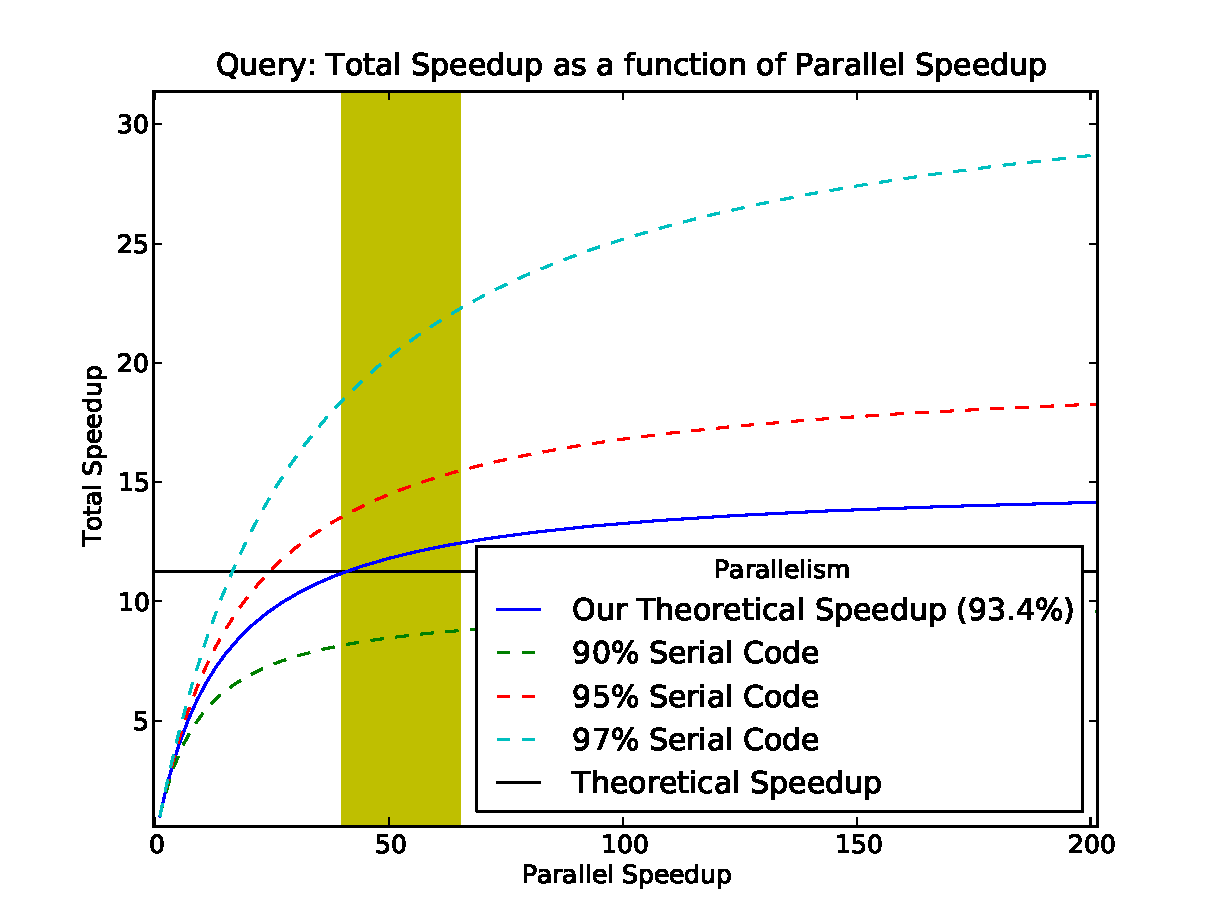
\includegraphics[scale=.30]{doc/speedupQuery}
\end{figure}
\end{frame}
\begin{frame}{First Attempt - Cardinality Mean Shift}
\begin{itemize}
 \item Partition data across nodes
 \item Count partition sizes
 \item Move datapoints toward large partitions
\end{itemize}
 \begin{figure}
  \centering 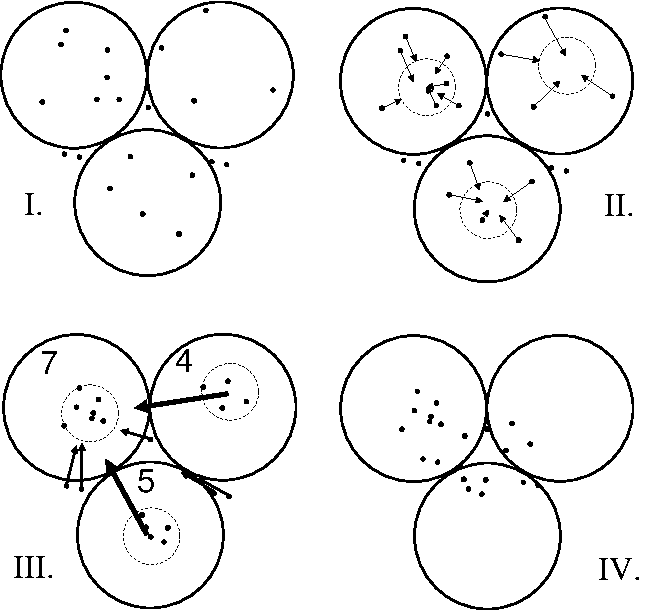
\includegraphics[scale=.30]{doc/cardshift}
\end{figure}
Unsuccessful due to too much communication and the ever present iterative structure.
\end{frame}
\begin{frame}{RPHash}
 \begin{itemize}
  \item Random Projection Hash Clustering
  \item Random Project vectors into a partitions of the Leech Lattice
  \item Count Lattice Partition Counts
  \item Accumulate partition counts across nodes($\Theta($log-reduce))
 \end{itemize}
\end{frame}
\begin{frame}{An Addition}
\begin{itemize}
  \item Project randomly multiple times for each point
  \item Projected point has a distribution about the optimal projection (blurring)
  \item Counting and key-mapping fit well in the map reduce framework
 \end{itemize}
  \begin{figure}
  \centering 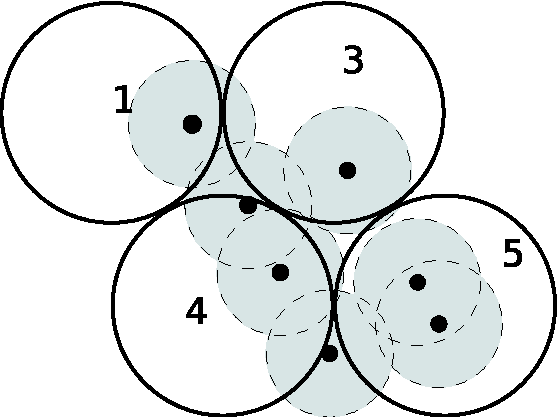
\includegraphics[scale=.50]{doc/randproj}
\end{figure}
\end{frame}

\begin{frame}{Preliminary Results: Sequential}
\begin{figure}
 
        \begin{subfigure}
	  \centering 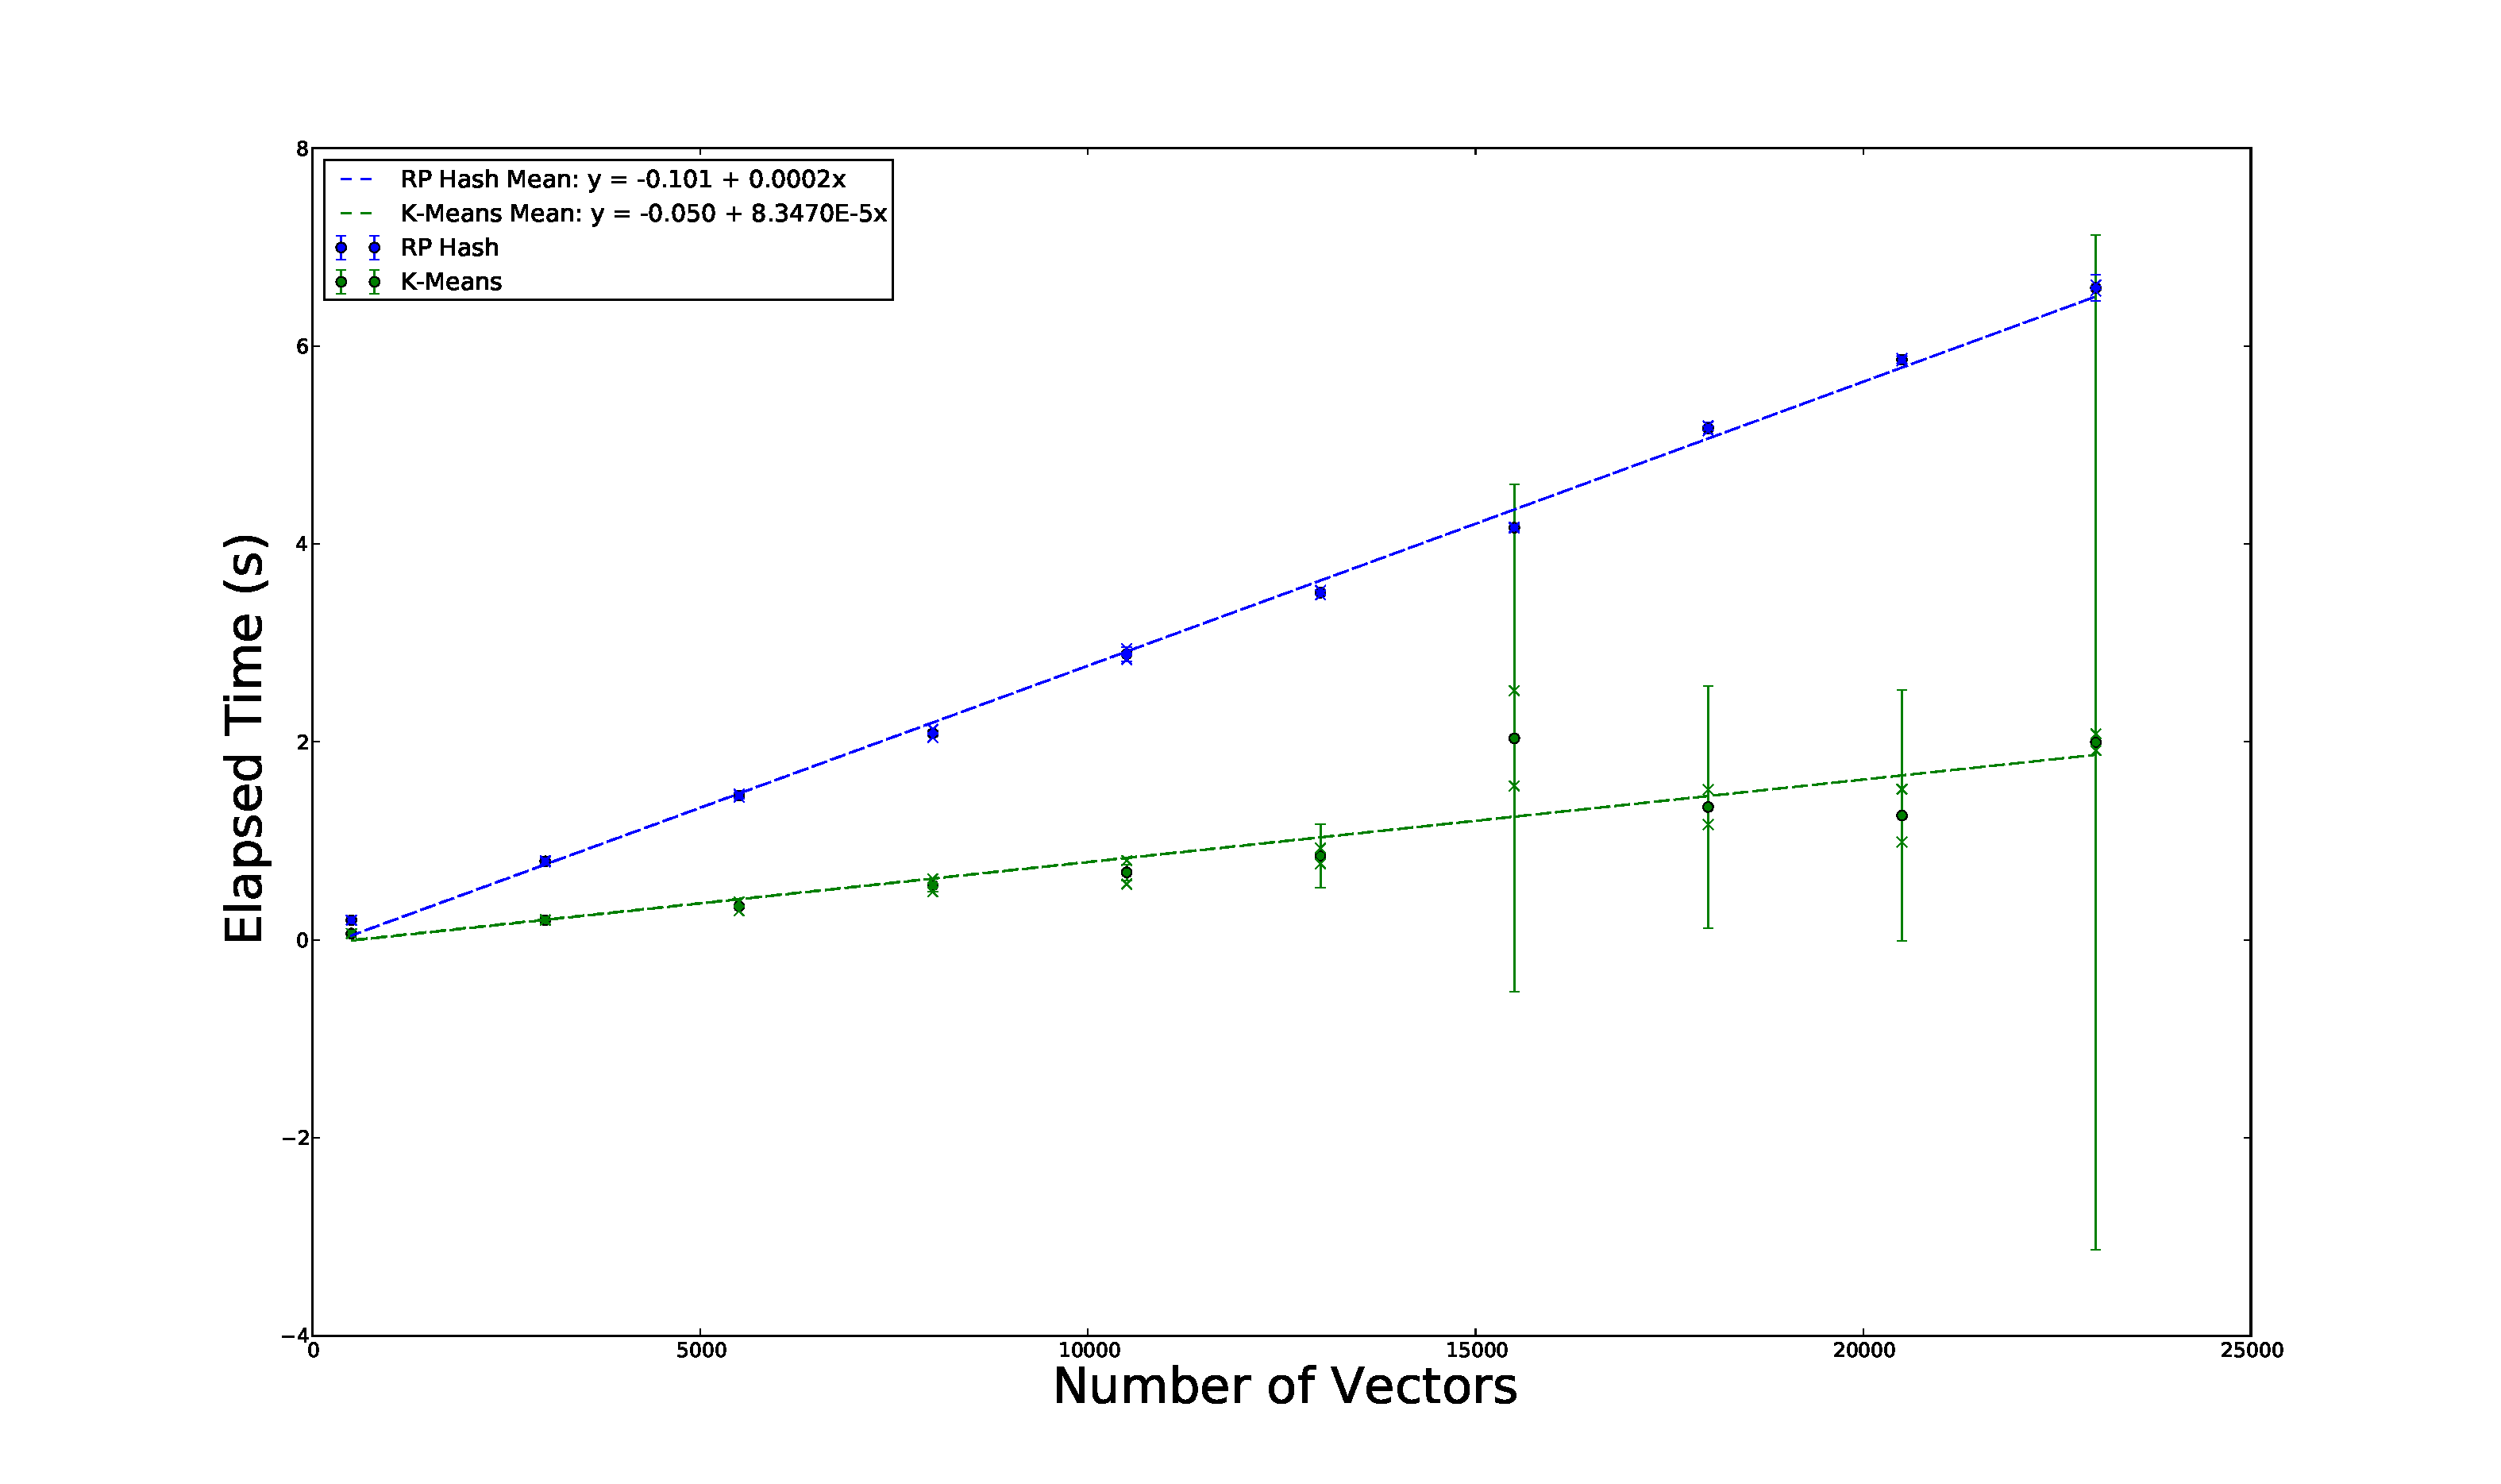
\includegraphics[scale=.10]{doc/TimevaryPart}
        \end{subfigure}
        \begin{subfigure}
                \centering 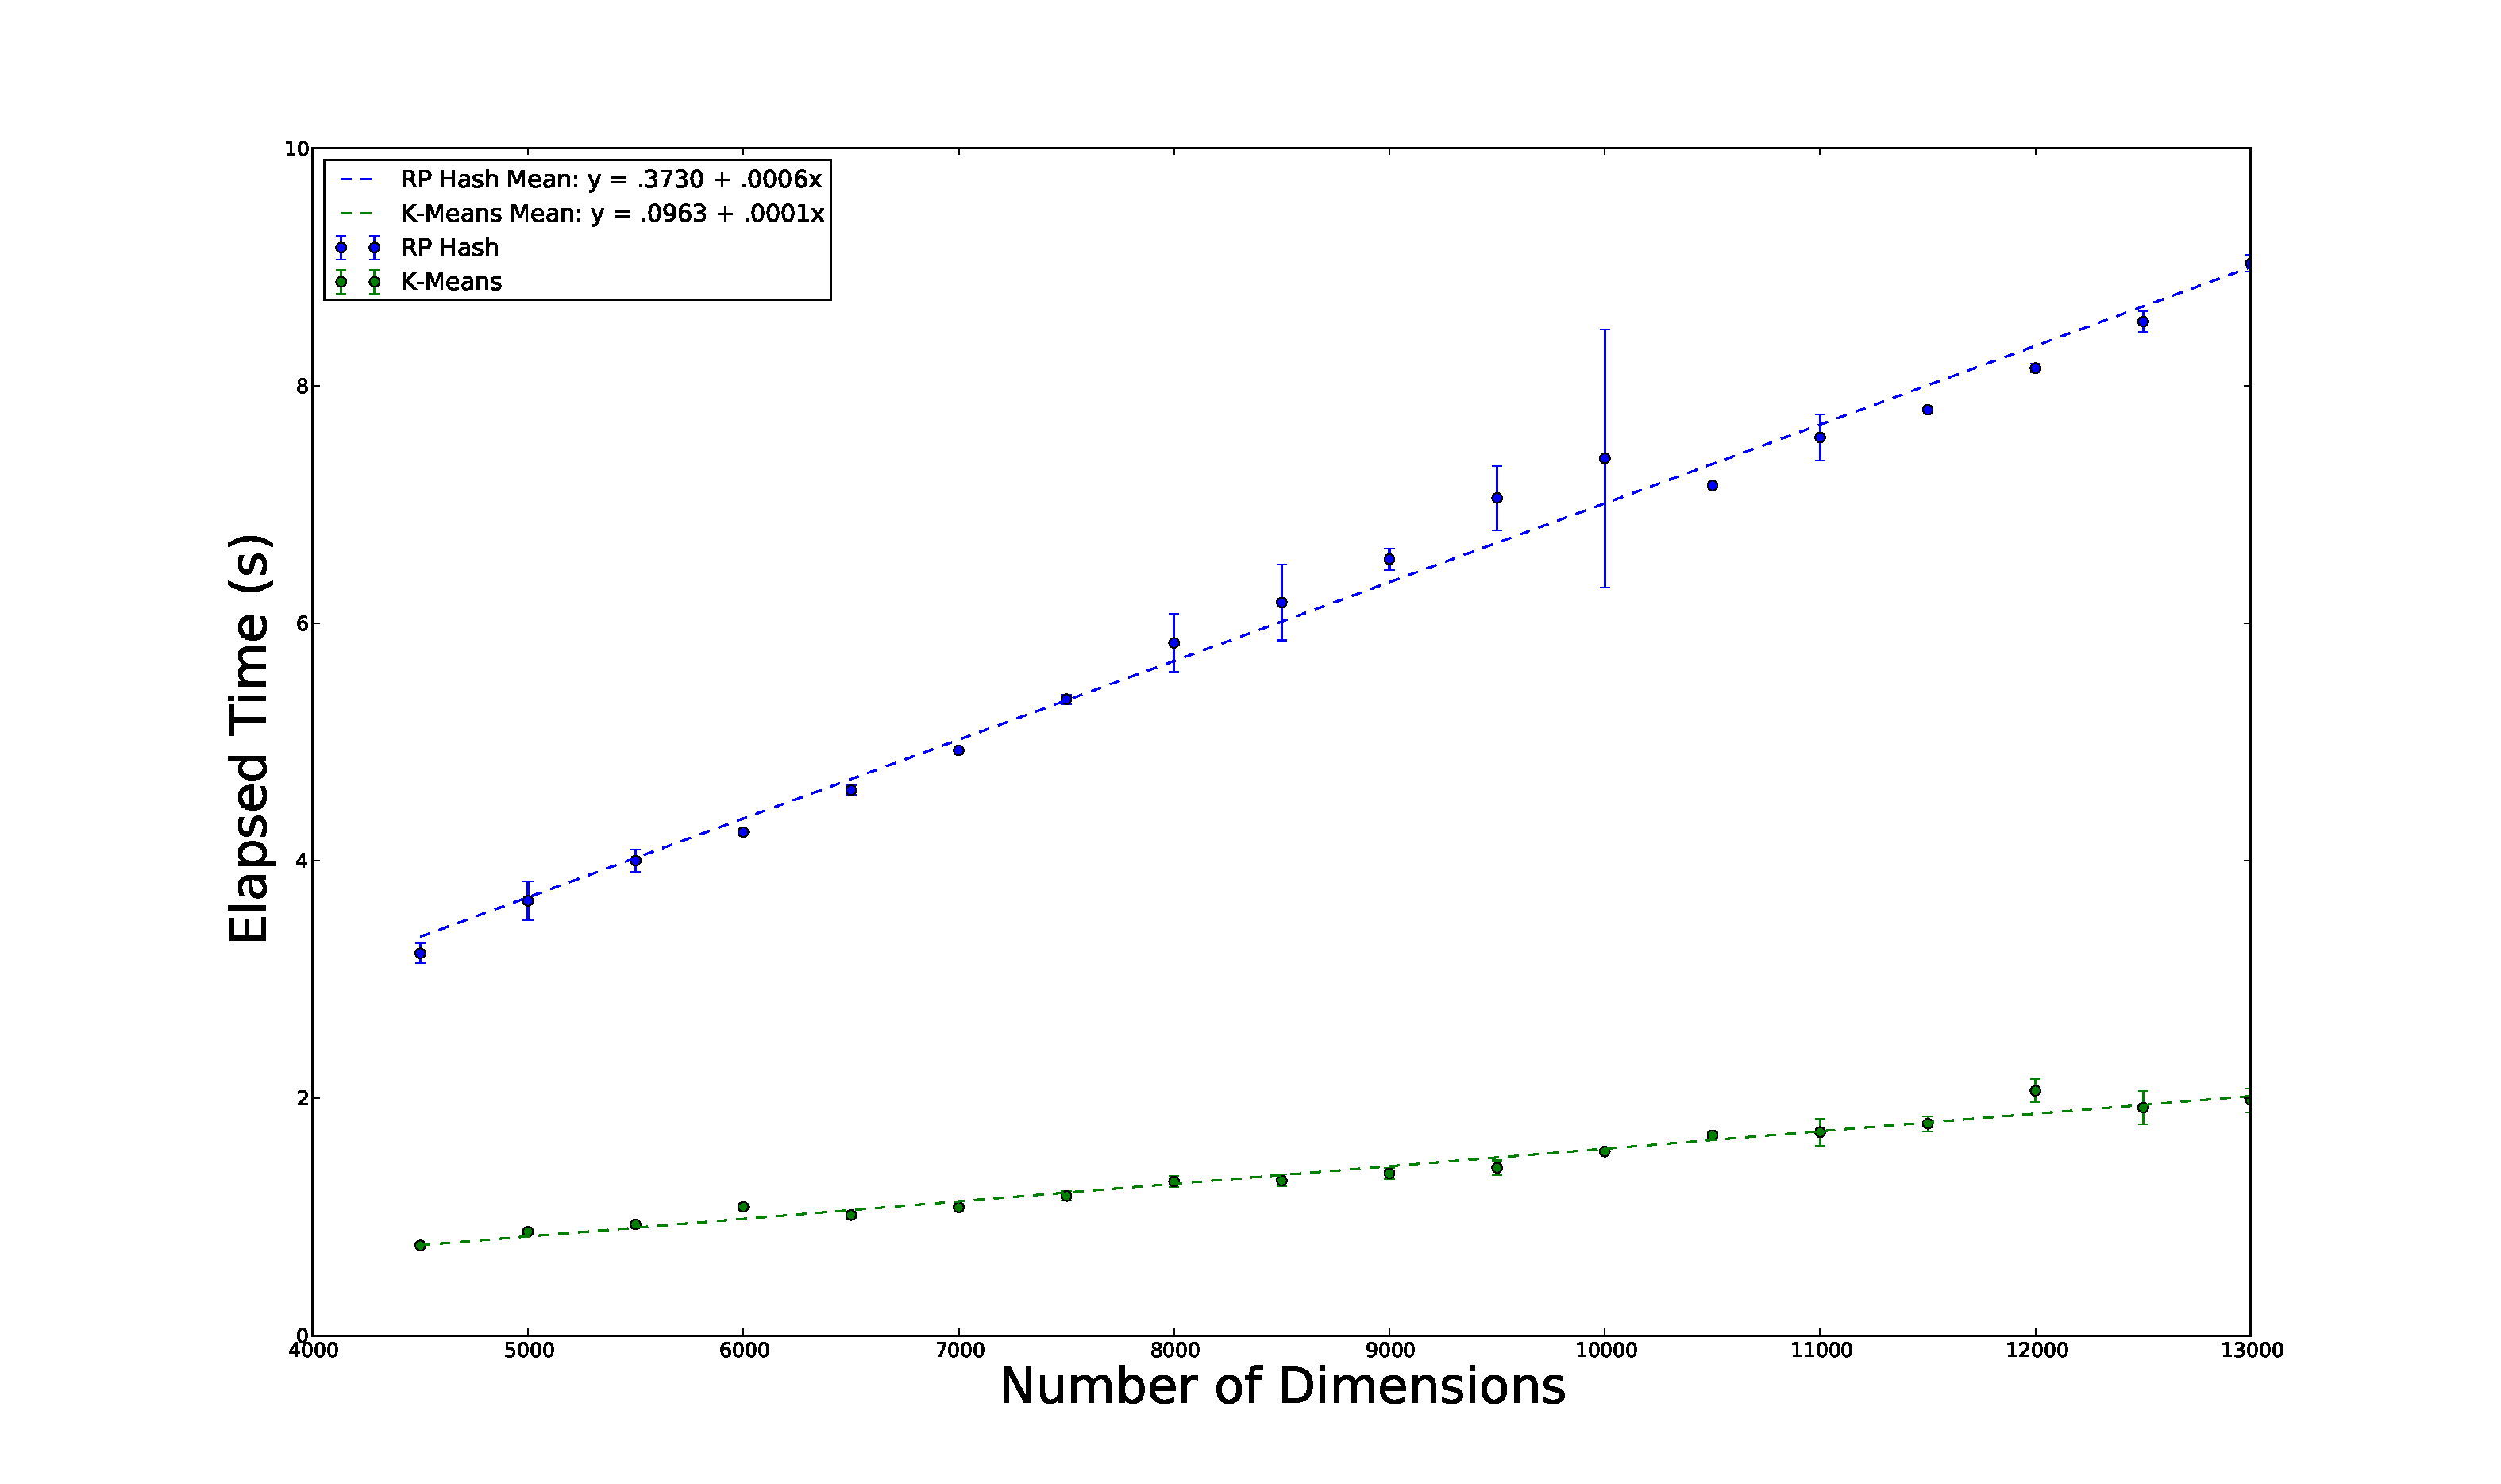
\includegraphics[scale=.10]{doc/TimevaryDim}
        \end{subfigure}
	  \caption{Computation Time for K-Means(green) and \emph{RPHash}(blue) 
               varying Vectors and Dimensions}\label{timecomplex}
\end{figure}
\begin{itemize}
 \item Worse than k-means!
 \item ok, since we are trading sequential complexity for parallel speedup
\end{itemize}

\end{frame}

\begin{frame}{RP for data obfuscation}
 \begin{itemize}
  \item RP is destructive mapping with possible application to deidentification attack prevention
  \item Important following infamous attacks
  \item Presidential Commison of WGS security\cite{presidential}
 \end{itemize}

$$ u = \sqrt{{\frac{n}{k}}}R_{d\rightarrow s}^Tv ,
v' = \sqrt{{\frac{k}{n}}}u^T R_{d\rightarrow s}^{-1}, $$
$$s(v,v') = ||v,v'||_{2}, $$
$$
\forall\{v,v'\} \in V , \exists {\hat{v}} \in V : s(v,v')>s(\hat{v},v) \text{ where } \hat{v}\neq v
$$
\end{frame}
\begin{frame}{Part 1 Conclusions}
 \begin{itemize}
  \item Ongoing research with NSF proposal being recommended for funding.
  \item Current subject of ongoing dissertation research
 \end{itemize}
\end{frame}
\begin{frame}{Part 2 BMI Session}
\begin{itemize}
 \item Worked with Prof. Medvedovic
 \item Learned about Gene enrichment and Gaussian Infinite Mixture Model
 \item Expectation Maximization(EM) in java for MLE of parameters (java)
 \item Attempt to parallelize GIMM directly on GPU
 \item Theano: CPU and GPU compiler for math in Python
 \item Elastic Cloud GIMM server backend
 \end{itemize}
\end{frame}
\begin{frame}{Enrichment in TreeView}
 \begin{figure}
  \centering 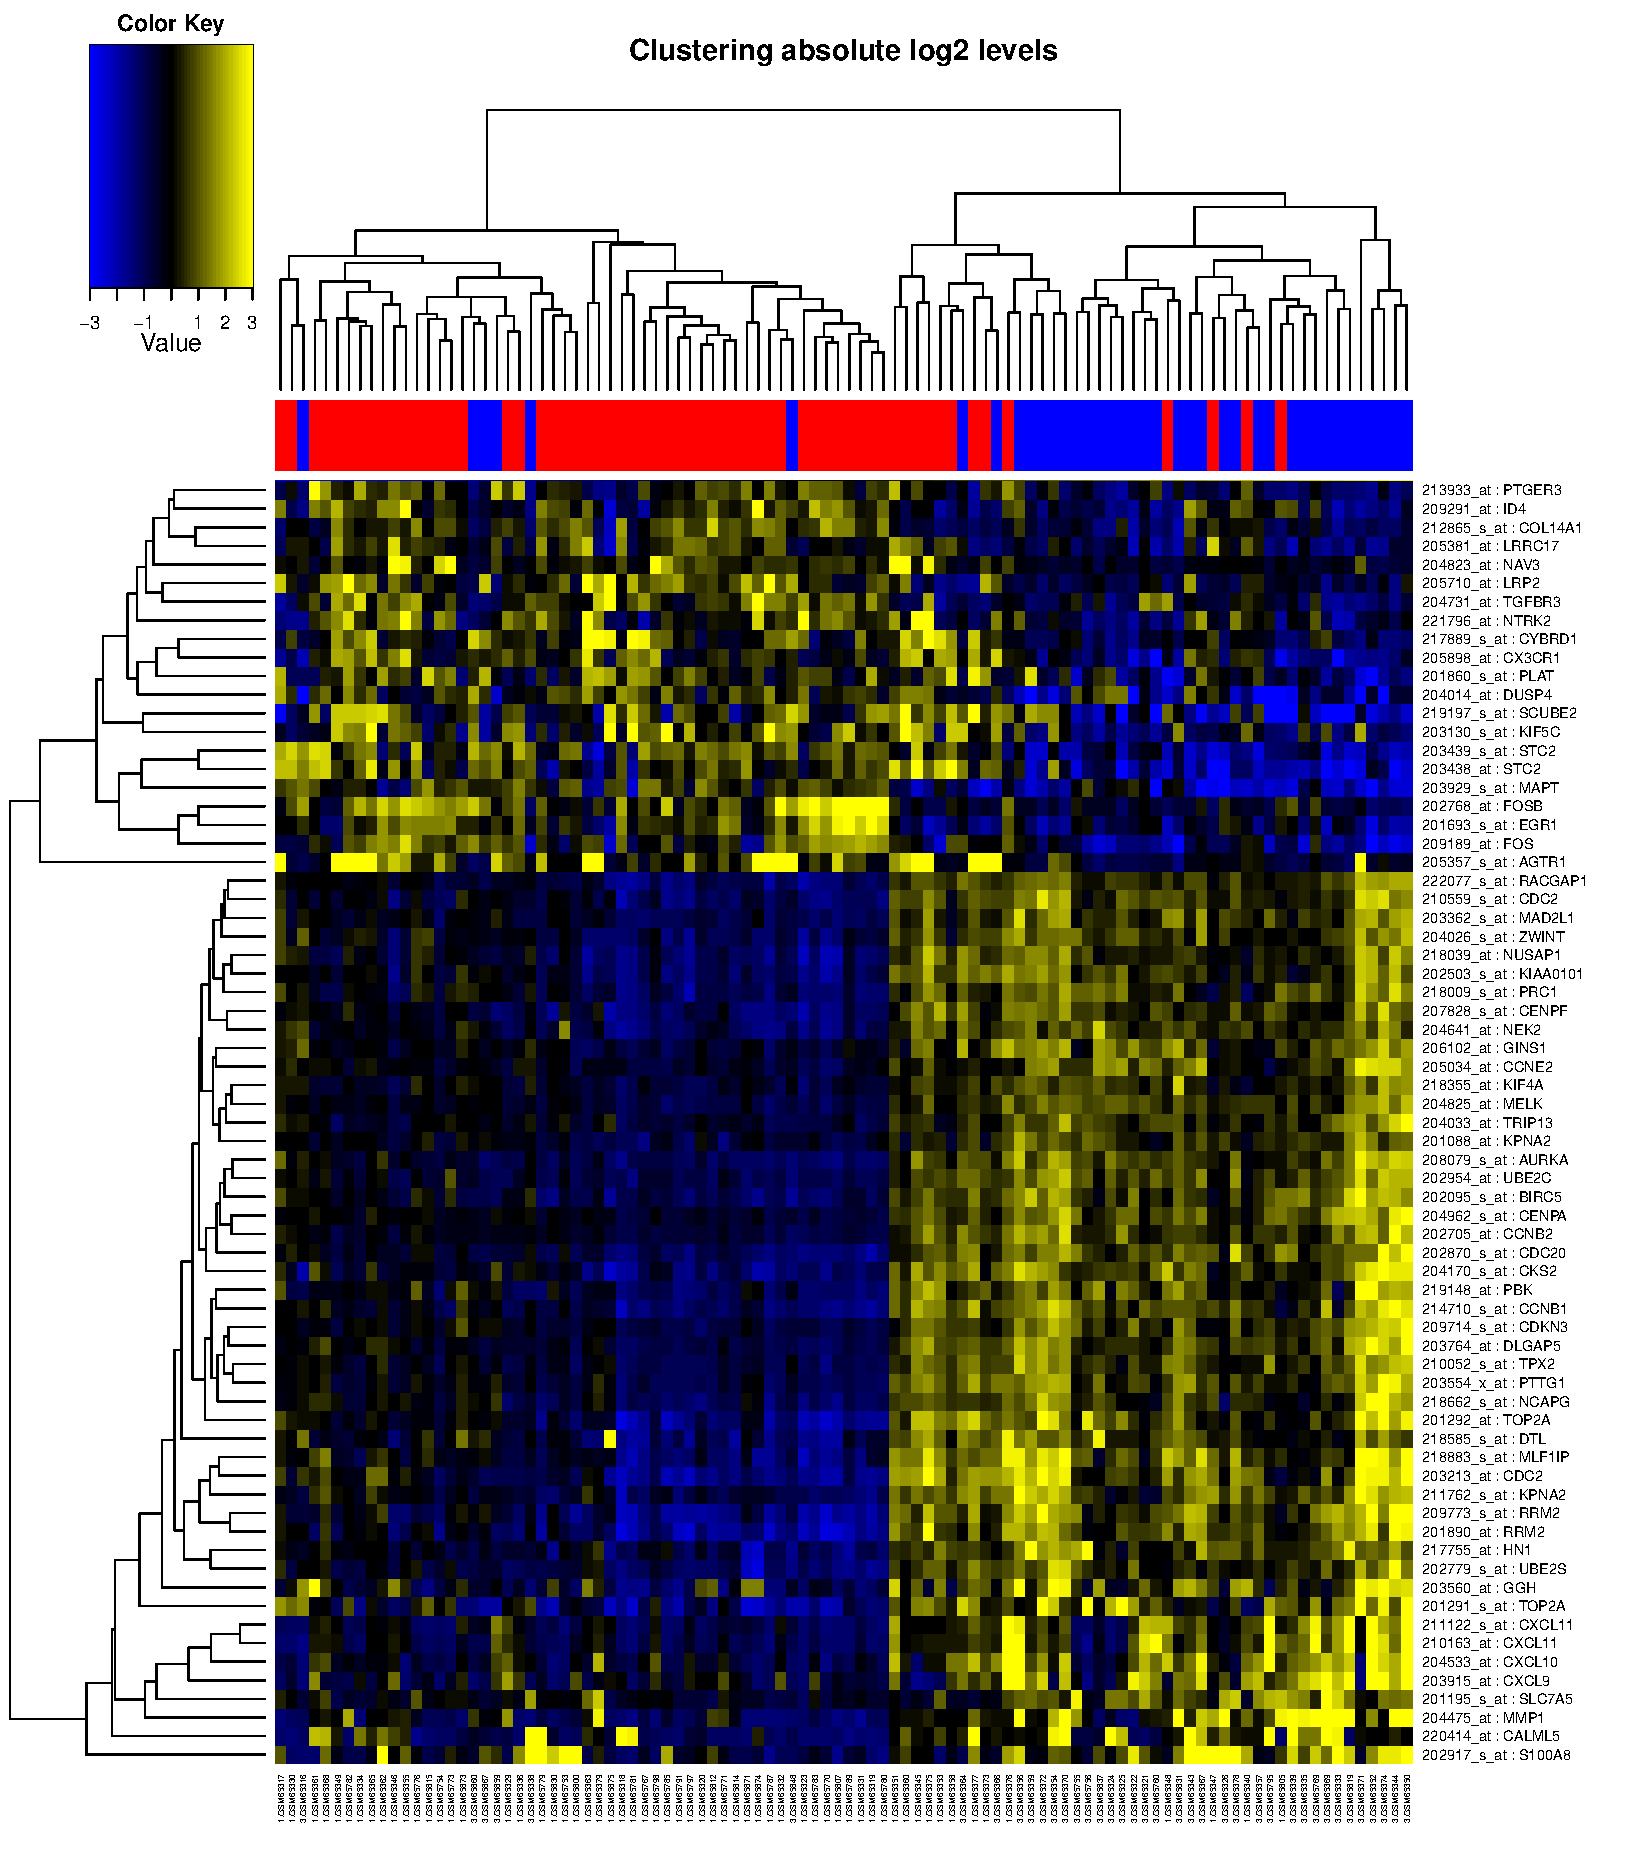
\includegraphics[scale=.20]{doc/diffexpress}
\end{figure}
\end{frame}
\begin{frame}{Faster than Fisher tests}
 \begin{itemize}
  \item Differential Expression is important, fisher's..
  \item MLE can approximate p-values via EM algorithm
  \item Developed a maximum-likelihood estimator in java, target hadoop
  \item Hadoop is a Map Reduce(MR) processing engine
  \item Mahout contains an MR optimized EM algorithm
  \item GIMM allows for mixture of prob. dist.
 \end{itemize}
\end{frame}

\begin{frame}{GIMM}
 Gaussian Infinite Mixture Model (sometimes IGMM)
 \begin{itemize}
  \item Instead of EM, GIMM uses Bayesian Estimation
  \item Gibb's is a Markov Chain Monte Carlo Algorithm
  \item Gibb's Sampling uses conjugate priors (Dirichlet, Inverse Wishart)
  \item Main Process is Sampling the Prior Distribution
 \end{itemize}
\end{frame}

\begin{frame}{GPGPU's have lots of ALUs}
\begin{figure}
  \centering 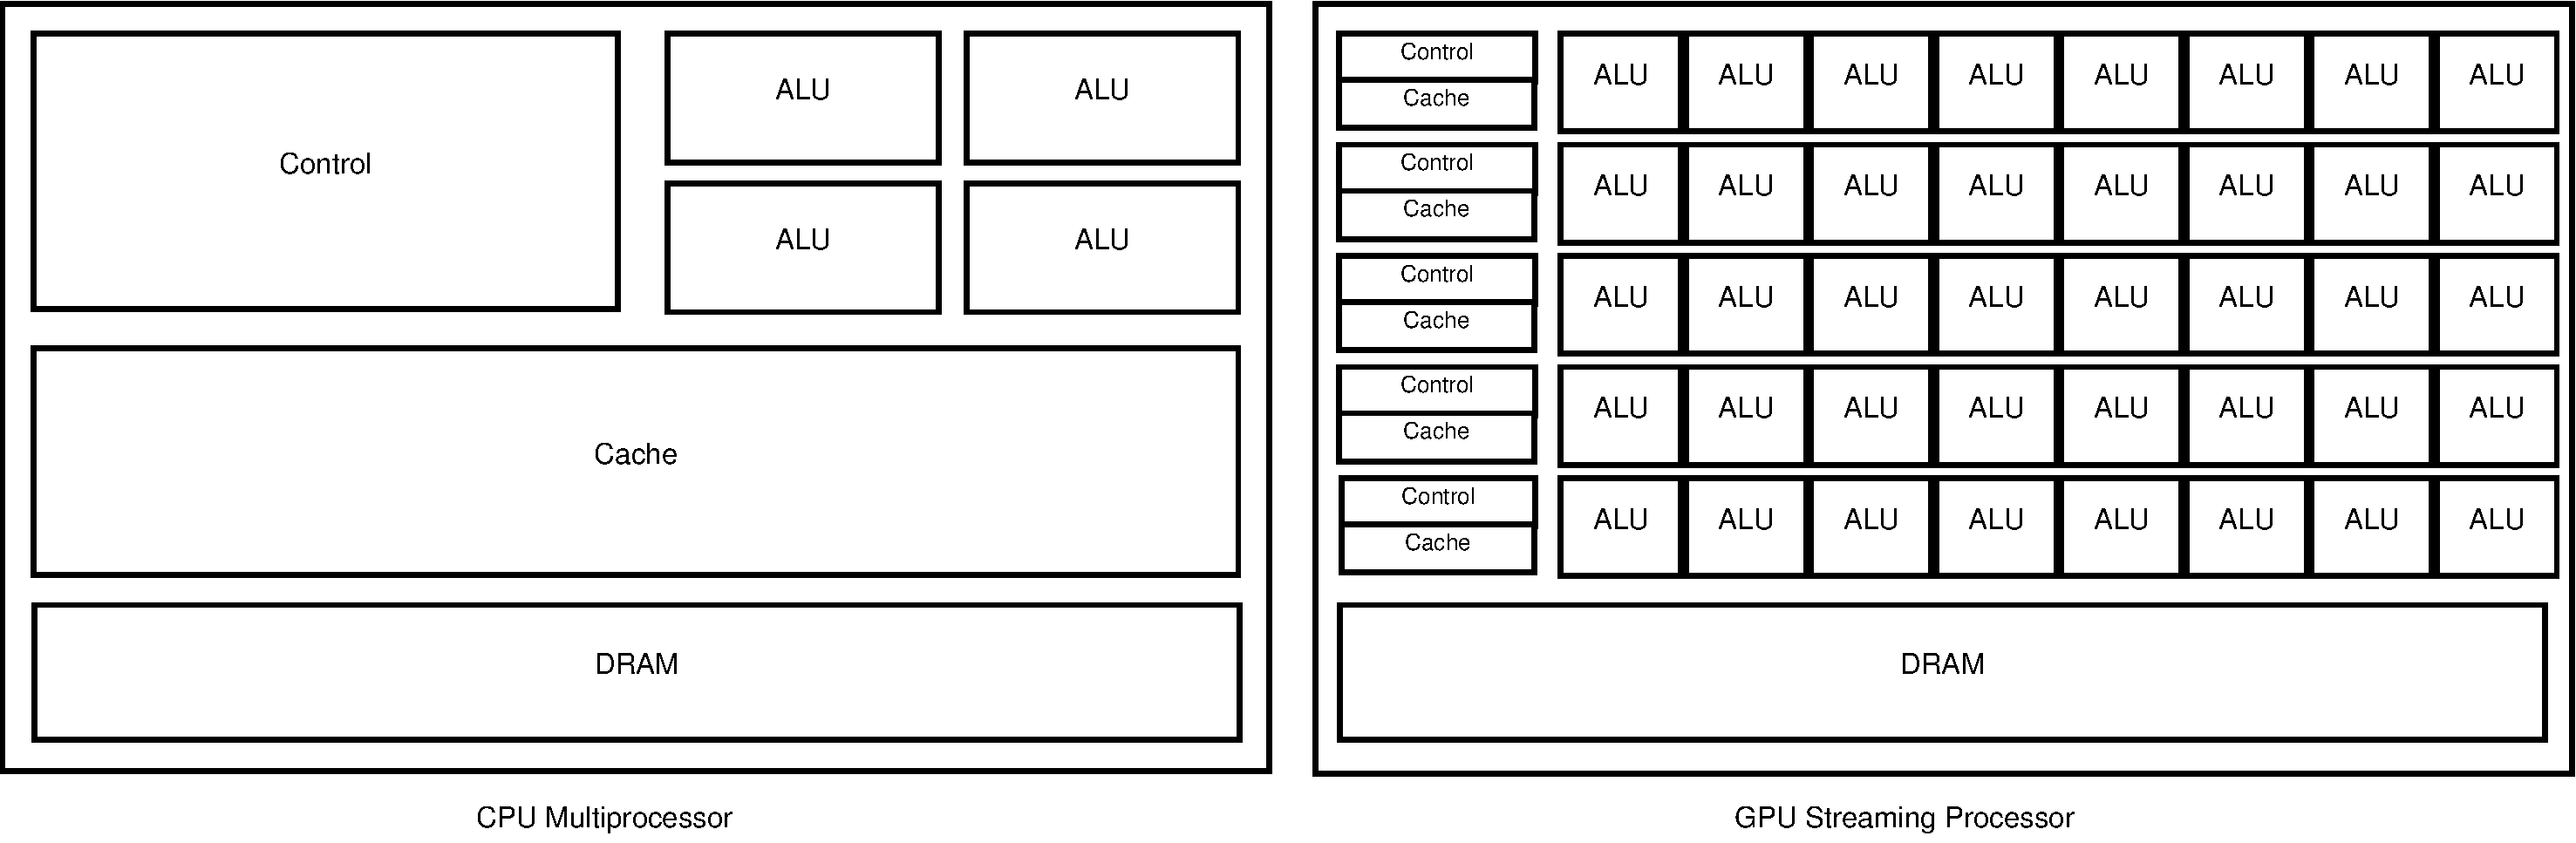
\includegraphics[scale=.20]{doc/GPUvCPUArch}
\end{figure}
\begin{itemize}
 \item More Arithmetic Logic Units Compared to Control Logic and Memory
 \item More common as more libraries leveraging GPU's are made available.
 \item NVIDIA implementation CUDA, also OpenCL for AMD
\end{itemize}
\end{frame}

\begin{frame}{GPGPU for R and GIMM}
  Before trying to implement directly, consider existing GPGPU 
  acceleration in R and Matlab.
  \begin{itemize}
   \item Matlab has most Lin Alg implemented in CUDA
   \item Also has keywords for accessing gpu cores
   \item R has HiPlar - similar to Matlab (Lin Alg, Matrix)
   \item R can be C so also have direct cuda implementations of code
   \item gimmR is a compiled binary, so not very useful directly.
  \end{itemize}
\end{frame}


\begin{frame}{GIMM Parallel}
\begin{figure}
  \centering 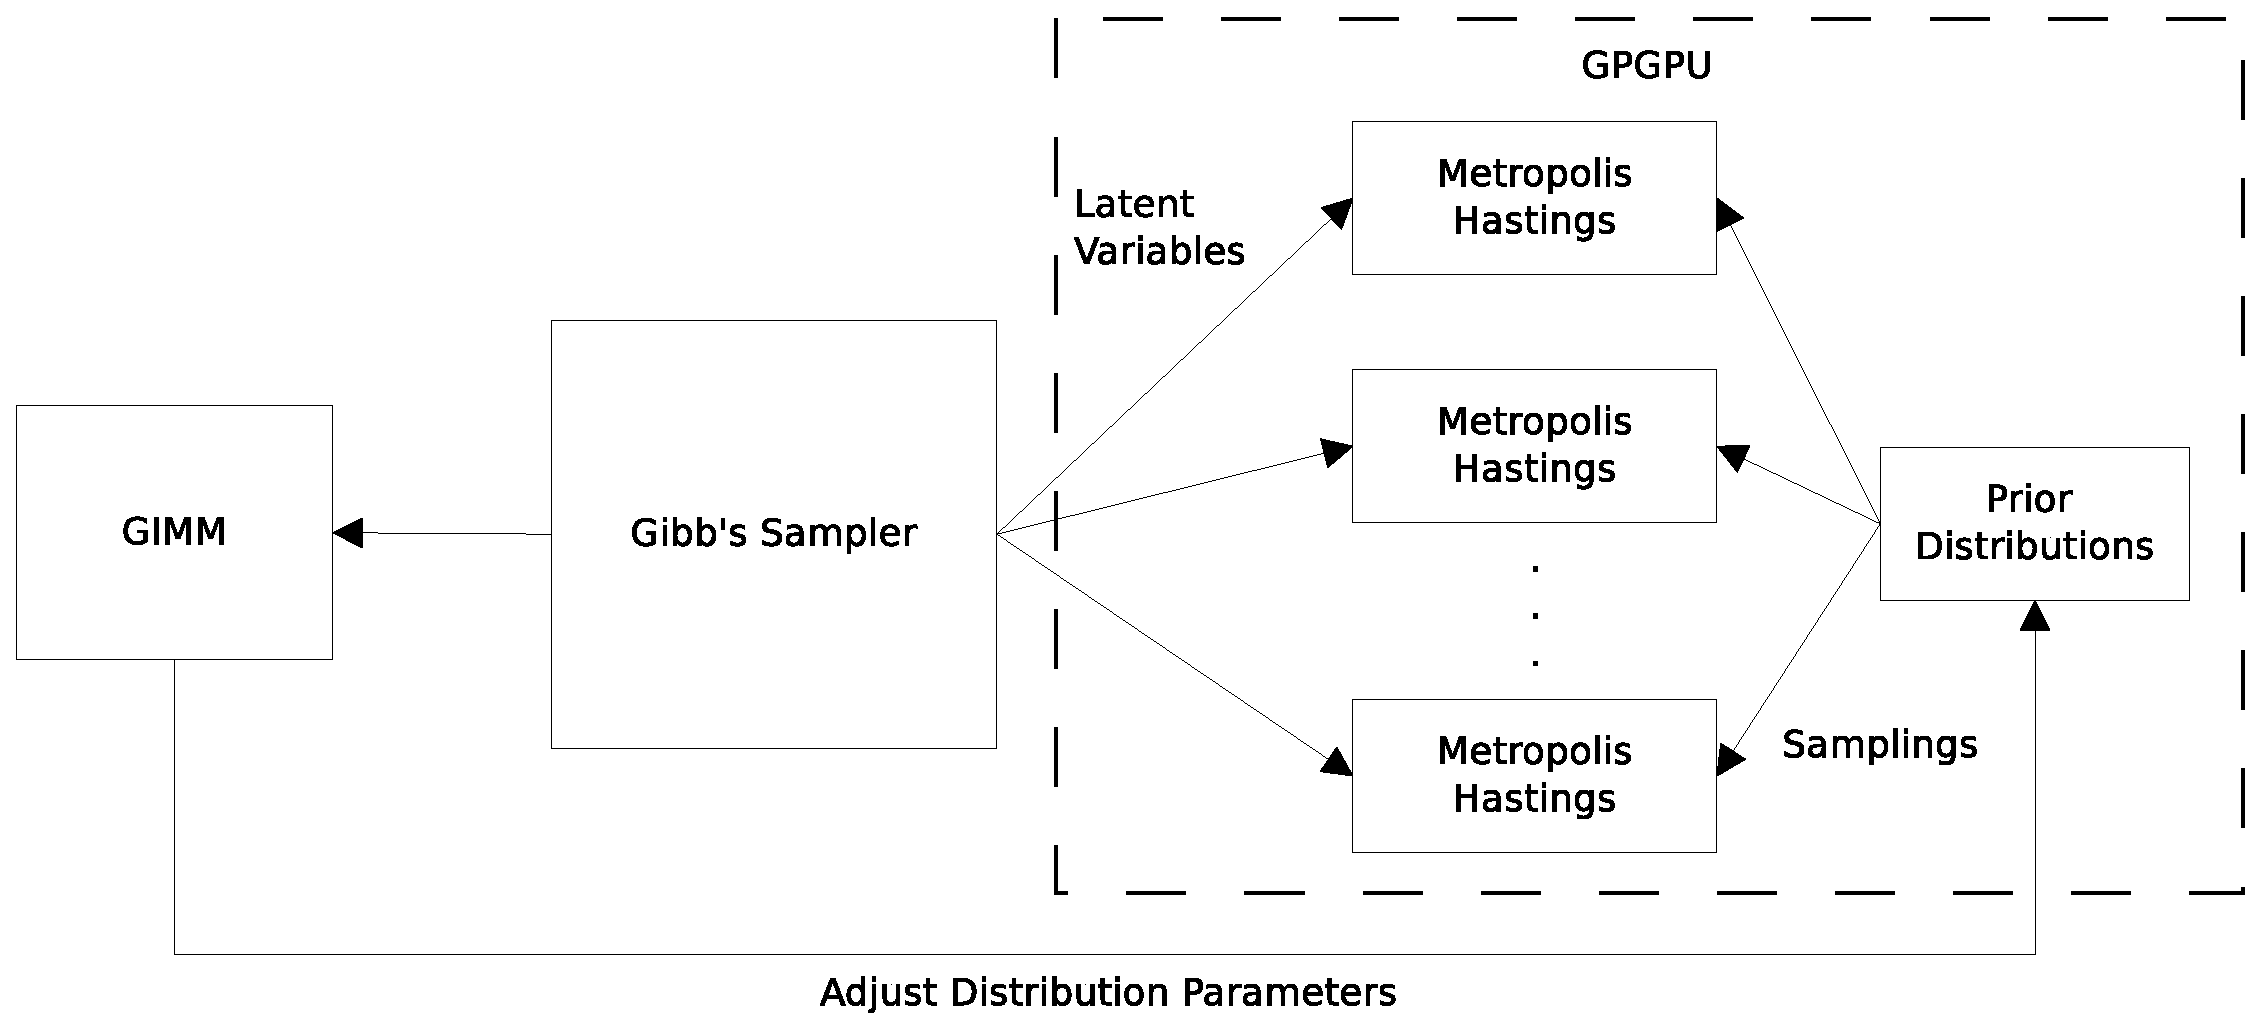
\includegraphics[scale=.20]{doc/GIMM}
\end{figure}
 \begin{itemize}
  \item Find parallelizable portions of GIMM (sampler)
  \item Most of the time spent generating samples
  \item Performance modeling this part in c and python
  \end{itemize}
  \end{frame}
  
 \begin{frame}{GIMM Parallel}
\begin{figure}
  \centering 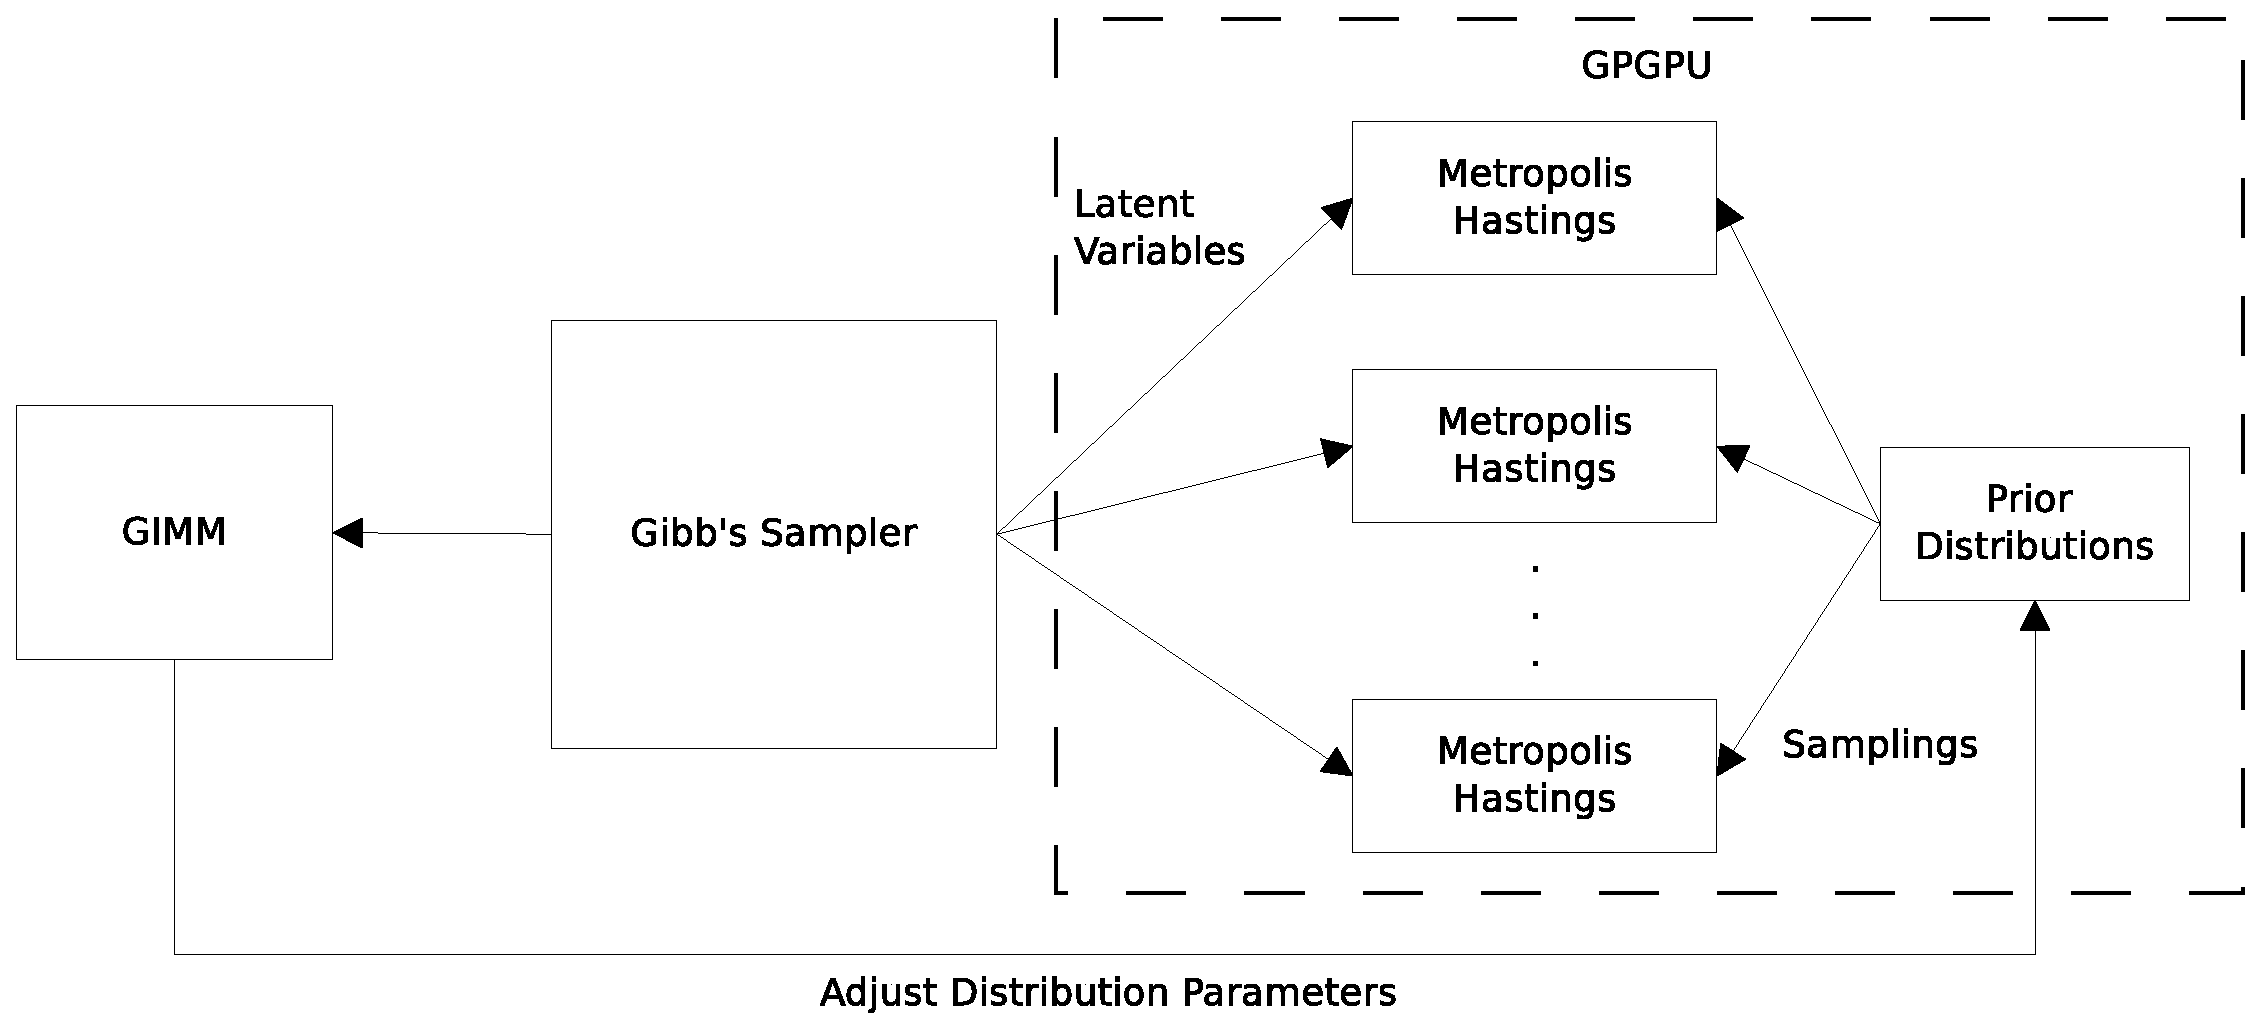
\includegraphics[scale=.20]{doc/GIMM}
\end{figure}
 \begin{itemize}
  \item Major Part is the Gibb's Sampler
  \item Can random distributions be sampled faster
  \item Fast gamma variate and Gaussian variates
  \item How do we overlap transfers to improve SPU occupancy and minimize sequential bottleneck
  \end{itemize}
\end{frame}

\begin{frame}{Fast Uniform Random Numbers}

 \begin{itemize}
  \item From GPU Gems Nvidia
  \item Implement a wallace pool prng
  \item Based on Walsh-Hadamard Matrix
  \item GPU-based Wallace generator provides a speedup of 26 times
 \end{itemize}
\end{frame}
  
\begin{frame}{GIMM Parallel}
 \begin{itemize}
  \item CUDA installation had many issues, but eventually mostly worked (glu libs were broken)
  \item A direct CUDA implementation with occupancy tuning would likely be optimal
  \item Could not fit inverse-wishart code into a single thread's memory
  \item Global memory is very slow
  \item Implemented simpler Gaussian sampler
  \item Issues with data transfer bottleneck are apparent in naive code
  \item A CUDA implementation is realizable but would require tuning.
 \end{itemize}
\end{frame}

\begin{frame}{ GIMM in Python}
  \begin{itemize}
  \item Scripting Languages are slow, why is this here?
  \item Pylab/Numpy Give fast access to c functions, like R
  \item Implement a Gibb's Sampler in python not very fast even with pypy (4x slower than c)
  \item But there are more inventive ways to interpret Python
  \end{itemize}
\end{frame}

\begin{frame}{Use Theano In Python}
Theano is a mathematic expression compiler
 \begin{itemize}
  \item Mathematical expressions are defined in python
  \item Theano uses many parallel optimized functions from BLAS to turn operations into SIMD vector operations
  \item Theano supports transparent CUDA (GPGPU) conversion
  \item overlapped data transfer is automatically performed by Theano 
 \end{itemize}
\end{frame}

\begin{frame}{Theano Performance Possibilities}
 \begin{figure}
  \centering 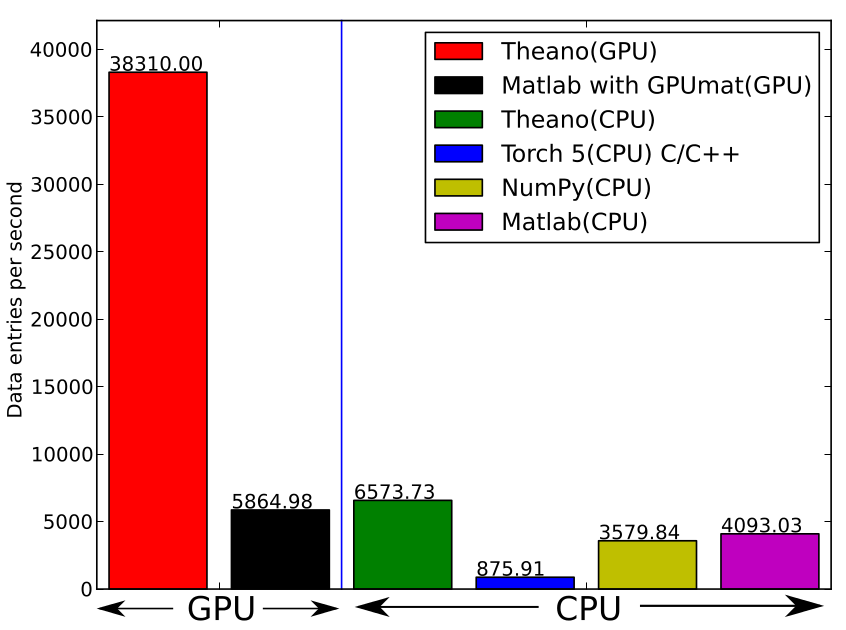
\includegraphics[scale=.30]{doc/theano}
  \end{figure}
  conference.scipy.org/scipy2010/slides/james\_bergstra\_theano.pdf
\end{frame}

\begin{frame}{Theano Use}

 \begin{itemize}
  \item Functions as python module
  \item Add static decorators to datatypes
  \item Convert function into expression graphs
  \item Compile expression graphs into optimized c or gpu code
 \end{itemize}
\end{frame}
\begin{frame}{Theano Performance Possibilities}
 \begin{figure}
 \begin{subfigure}
    \centering 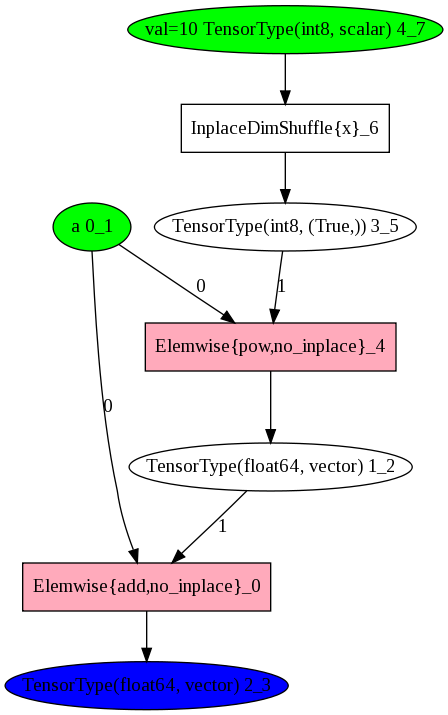
\includegraphics[scale=.20]{doc/fgraph}
 \end{subfigure}
\begin{subfigure}
  \centering 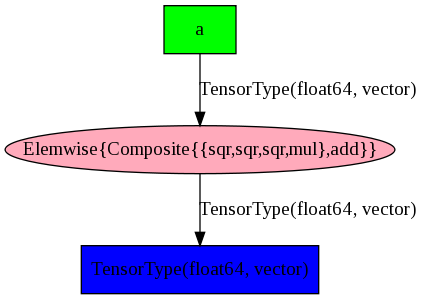
\includegraphics[scale=.20]{doc/fgraphop}
  \end{subfigure}
  \caption{(http://deeplearning.net/software/theano/tutorial/symbolic\_graphs.html)}
  \end{figure}
  \end{frame}
  

\begin{frame}{Performance Profile IGMM}
   \begin{figure}
  \centering 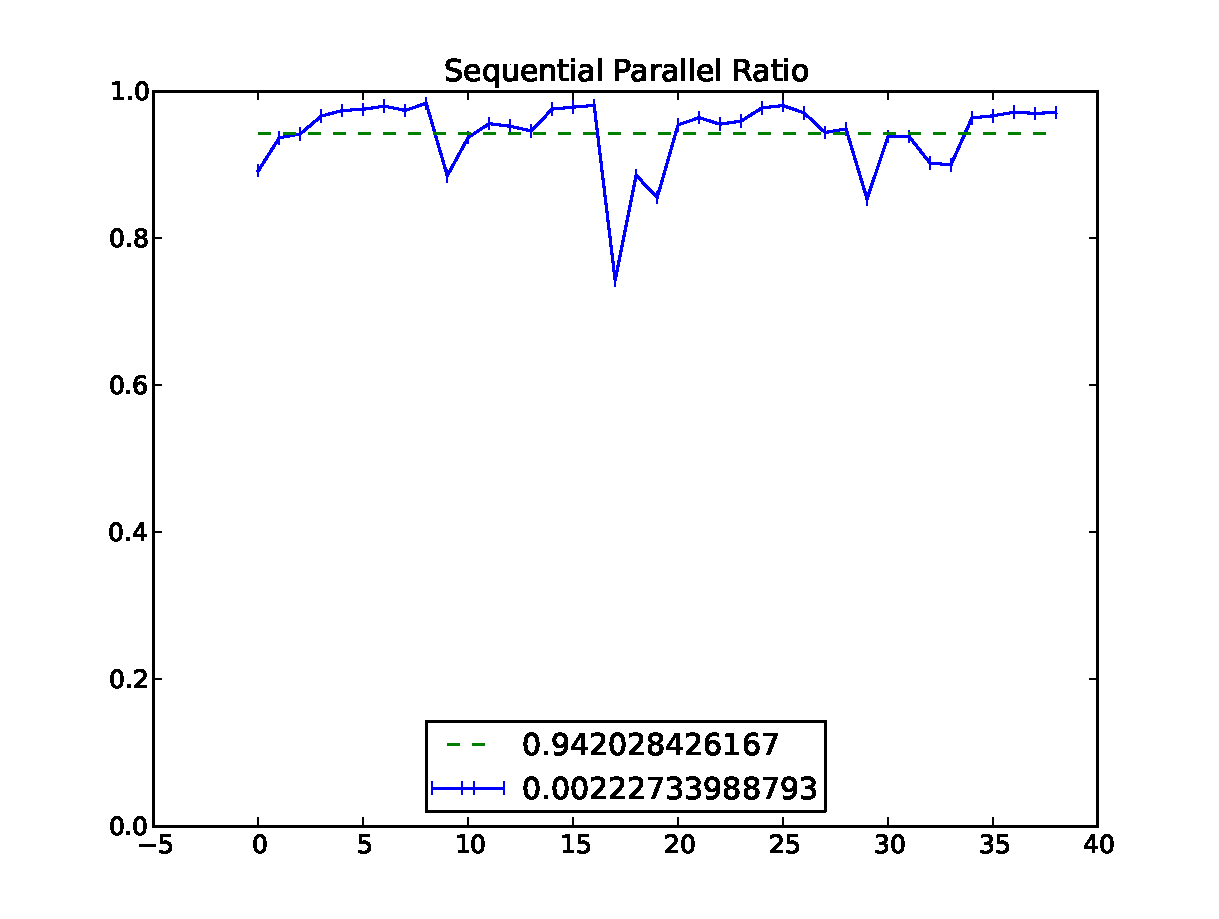
\includegraphics[scale=.30]{doc/seqpar}
  \end{figure}
  \begin{itemize}
   \item Majority of processing occurs in the pdf generation
   \item 94.2\% can be sped up by focusing here
   \item pdf generation is naively parallel
  \end{itemize}
\end{frame}

\begin{frame}{Applying Amdahl's Law}
   \begin{figure}
  \centering 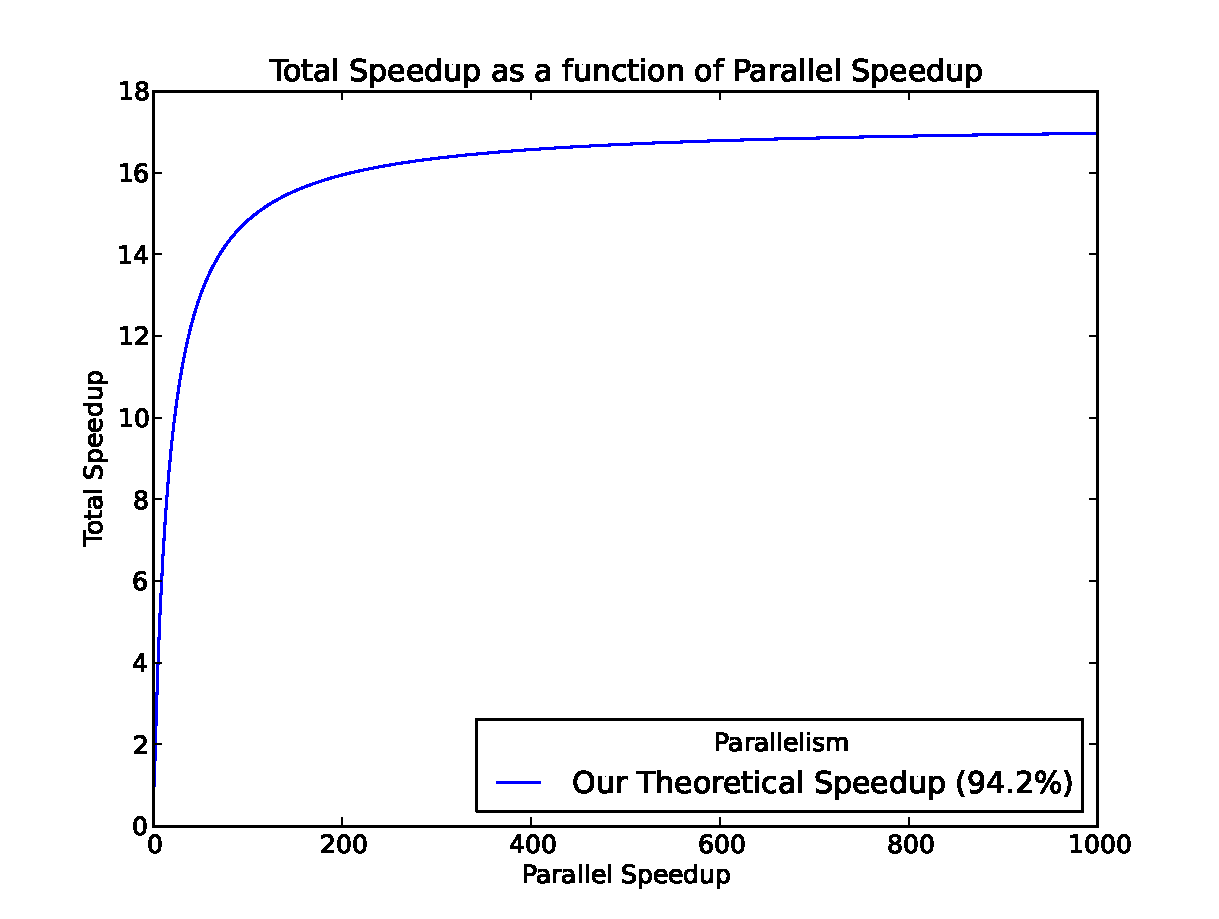
\includegraphics[scale=.40]{doc/speedup}
  \end{figure}
Applying Amdahl's Law on 94.2\% sequential to parallel ratio.
\end{frame}

\begin{frame}{Theano GPU vs CPU}
Real World Speedup?
   \begin{figure}
   \begin{subfigure}
  \centering 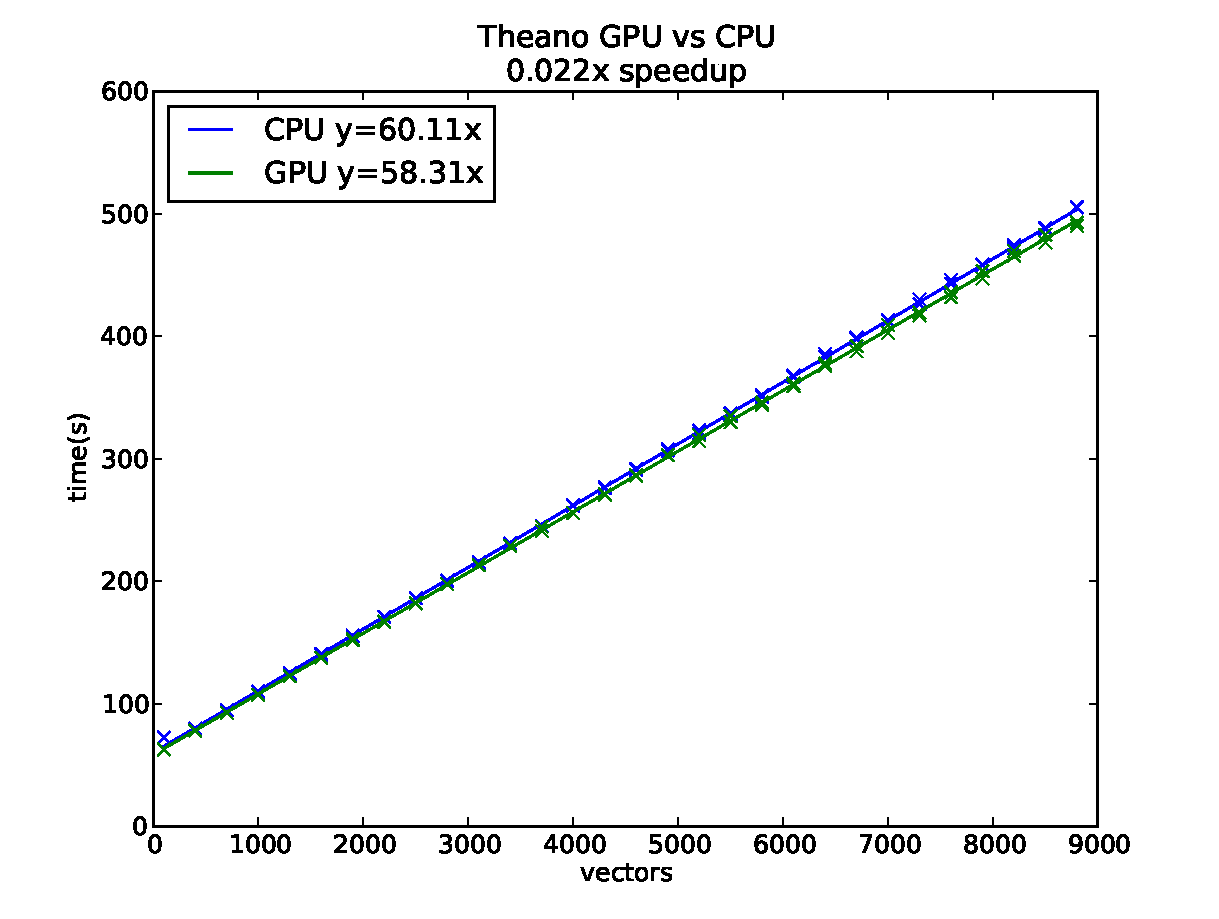
\includegraphics[scale=.25]{doc/gpucpu}
  \end{subfigure}
  \begin{subfigure}
  \centering 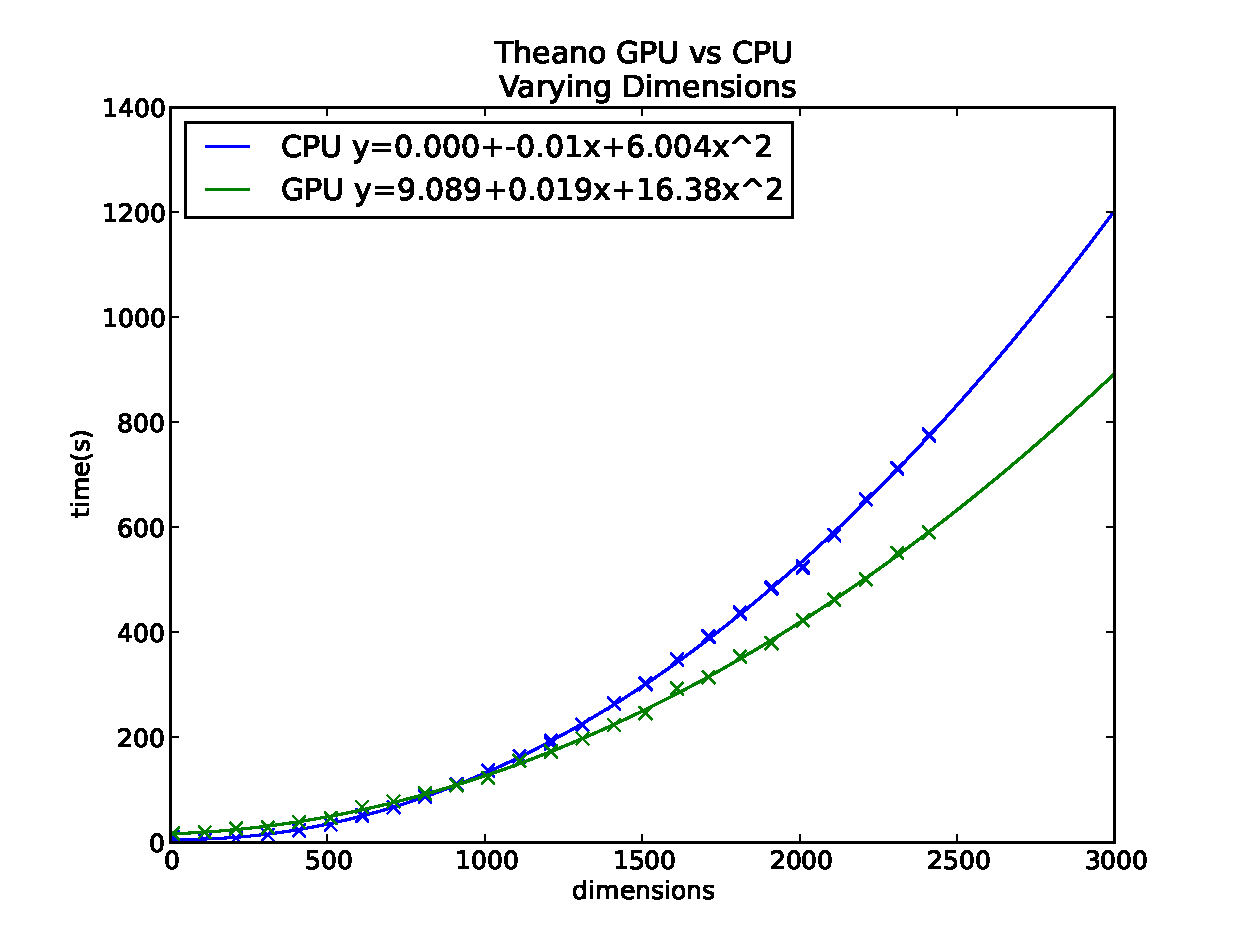
\includegraphics[scale=.25]{doc/gpucpuD}
   \end{subfigure}
   \begin{itemize}
    \item Cost of JIT and cpu$\rightarrow$gpu transfer times
    \item Dimension calls are vector ops in Theano,
    \begin{itemize}
      \item More data per DMA transfer cycle
     \end{itemize}
   \end{itemize}
  \end{figure}

\end{frame}

 
\begin{frame}{A step back to see what is really needed}
 \begin{itemize}
  \item Individual problems aren't really big data problems
  \item The issue is more of user load balancing and resource allocation (and unallocation)
  \item Load balancing independent jobs is parallel
  \item This suggested utilizing elastic computing services
 \end{itemize}
\end{frame}

\begin{frame}{WebGimm}
 \begin{figure}
  \centering 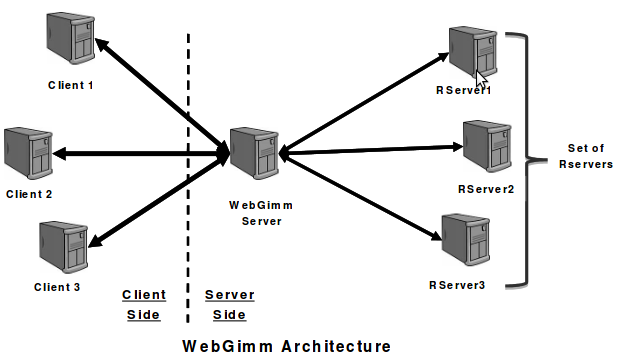
\includegraphics[scale=.30]{doc/webgimm}
\end{figure}
eh3.uc.edu/gimm/webgimm/files/deployment.pdf
 \begin{itemize}
  \item A webserver and backend processing model
  \item GIMM server backends exist but are fixed to physical available machines
  \item Elastic cloud services can spin up an down lxc containers as needed
 \end{itemize}
 \end{frame}
 
 \begin{frame}{Docker and LXC}
    \begin{figure}
  \centering 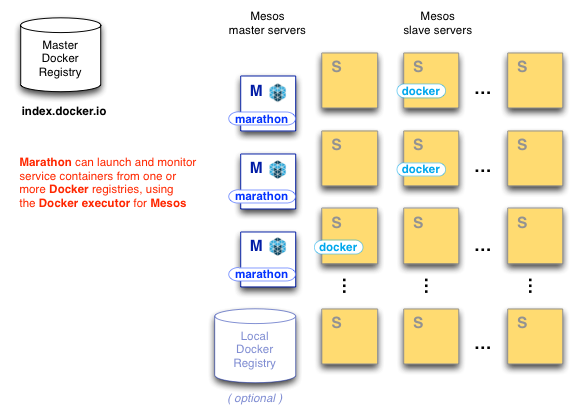
\includegraphics[scale=.30]{doc/mesos}
  \end{figure}
  tctechcrunch2011.files.wordpress.com/2013/09/mesos-docker-1.png
  \begin{itemize}
   \item Created a linux container with the GIMM server modules for dynamic creation
  \end{itemize}
 \end{frame}
 
  \begin{frame}{Distributed Frameworks}
  \begin{itemize}
    \item Attempted to setup internal cluster
    \item Attempts with Mesos, Cloudera and Pivotal phd could not be properly configured
    \item More custom method with just lxc and standard installations
    \end{itemize}
  \end{frame}
   \begin{frame}{Work In Progress}
  \begin{itemize}
   \item Setting up docker containers
   \item Automating creation and destruction of containers
   \item Updating WebGimm interface to control container creation
   \item Security of creation credentials 
  \end{itemize}
  \end{frame}
 \begin{frame}{Conclusions}
  \begin{itemize}
   \item Attempts to find more efficient parallel implementations of GIMM proved difficult
   \item Some methods are promising such as Theano
   \item The Container of the GIMM Server could very likely be launched in an elastic cloud for dynamic resource allocation, or internal to a University network
  \end{itemize}
 \end{frame}
 \bibliography{refs}
\end{document}
